\chapter{Scalable MoC-based Application Learning}
\label{cha:ch5}
To encompass the built-in intelligence and realtime processing capabilities of CPS within efficient computing and communication powers, it is of primary importance to understand the task structure of CPS applications, their computational and communication requirements and data access patterns.  While the exact structure and dynamic dependencies of CPS applications cannot be fully predicted, it is crucial to develop a novel application profiling framework to learn the inter-dependency among application tasks for capture of the characteristics of computation and communication workloads, allowing maximized exploration of fine-grain parallelism and concurrency for the design of an optimized NoC-based platform providing on-board real-time processing capabilities. To ensure a \textit{fast} and \textit{unbiased evaluation} of NoC-based many-core designs for CPS applications . These benchmarks must: (\textit{i}) preserve the dependency patterns and traffic behavior of real applications; (\textit{ii}) be scalable in terms of size, degree of spatio-temporal dependency, and amount of traffic load so that they provide a sufficient set of stressing test cases for the heterogeneous large-scale NoC architectures. Current application-based benchmark suites, synthetic task graphs, and trace-based benchmark suites do not concomitantly satisfy all the above-mentioned properties. Although certain application-based benchmark suites (e.g., Parsec~\cite{bienia08characterizationreport}, Splash-2~\cite{woo1995splash}) preserve the high-fidelity of the performance evaluation under a measuring framework with full architectural and operating system details, their applicability to large-scale NoCs presents the following limitations:\\
\noindent \textbf{\textit{i})} Application-based benchmarks may not always prove useful in measuring NoC performance as their generation may focus on representative sets of applications for parallelism exploration, i.e., weak cross-task data dependencies. For instance, only a small portion of collected applications in Parsec and Splash-2 exhibit significant inter-processes data dependencies~\cite{barrow2009communication}. Therefore, they have limited effectiveness when testing the stress endurance of NoC, thus posing critical challenges to offering performance guarantees under extreme situations. Such a stress test is essential for a NoC design with predictable performance and ensured Quality-of-Service(QoS).\\
\noindent \textbf{\textit{ii})} Application-based benchmark suites are not portable to a wide spectrum of architectures with rich heterogeneities. They usually maintain a relative fixed set of applications based on a specific machine model. For instance, Parsec is assuming a homogeneous chip multiprocessor (CMP) system with shared memory while Splash-2 adopts a distributed shared memory (DSM) model~\cite{bienia2008parsec}. Such assumptions limit their applicability to the evaluation of NoC in emerging heterogeneous systems, e.g., multiprocessor SoC(MPSoC) or hybrid CPU/GPU/FPGA system.\\
\noindent \textbf{\textit{iii})} Application-based benchmark suites require costly simulations. In spite of their good fidelity, full-system simulations are necessary for using these benchmarks, which require extended simulation time, e.g., on the order of days or weeks, depending on the level of simulation detail, architecture size, and the duration of the application region of interest. The long iteration cycle makes design-space exploration very difficult. Such an iteration could be even more time-consuming considering the non-deterministic impact on the full-system behavior (e.g., scheduling, synchronization or execution pathways ~\cite{alameldeen2003variability}) caused by changes in NoC designs.\\
\indent Synthetic benchmark suites are designed based on either task graphs that are statically extracted from applications (e.g., source code analysis)~\cite{pekkarinen2011set} or use stochastic models assuming a certain class of data generation processes (e.g., Poisson process)~\cite{dally2004principles}. In contrast with the full-system simulations, the simulation time is greatly reduced due to simplified system details. Despite their fastness, none of the approaches is able to mimic the spatio-temporal behaviors of real application communications. The stochastic model-based traffic synthesis assumes each data generation process is independent and can be fully characterized by a set of parameters associated with the assumed stochastic model (e.g., the rate of a Poisson process). In this sense, synthetic benchmarks can be easily scaled to test NoCs of arbitrary size, topology and dimensionality, but they can lead to unrealistic or biased evaluations as a result of the disconnection with the  real applications.\\
\indent Static task graph-based benchmarks overcome the drawback of stochastic synthetic benchmarks by capturing some degree of the realistic spatio-temporal task dependencies. Static task graphs are determined via analyzing the source codes of application at compilation time. Computation and synchronization tasks are identified and represented as nodes in the resulting graph. The inter-task dependencies are captured by constructing directed links between a pair of task nodes. Therefore, the task structure of the application is naturally encoded by the size, composition and topology of the task graph. However, static task graph also places significant limitations on its applicability as all tasks and dependencies must be known up front. However, in many cases, the inter-task data dependencies can only be fully known during execution time. To illustrate this, we show a simple segment of C-style pseudo codes in Figure 1 where the types of task performed cannot be decided at compilation time but based on the choice of user input. As a result, statically extracted task graph is incapable of handling problems where the task breakdown, i.e., tasks and their dependencies, is only known at runtime, where a dynamically learned task graph during the execution time is thus required.\\
\indent Trace-driven benchmark suites collect inter-core communication traces during the application execution under a specific full-system setting. The traffic trace is then used as the input to drive the target NoC architecture for performance evaluation. This technique serves as a trade-off between the application-based benchmarks of high fidelity at the expense of simulation cost and the synthetic benchmarks. Recent trace-driven benchmarks like Netrace~\cite{hestness2010netrace} also consider inter-task data-dependencies for the preservation of real application behaviors, which improves their fidelity further. However, the trace-driven benchmarks are useful as long as the target architecture of interest coincides with that used for trace extraction. Otherwise, a trace recollection process through full-system simulation is required.\\
\begin{figure}%[htb]
  \centering
  % Requires \usepackage{graphicx}
 % \epsfig{file=t_calc.eps}
  \includegraphics[width=0.75\columnwidth]{dep.eps}
  \vskip -3mm
  \caption{A simple case where data dependencies can be known only at execution time as user input determines both data and the type of task to be performed. }
  \label{fig:CODE}
  \vskip -6mm
\end{figure}
\indent Based on these observations, we address the NoC benchmark synthesis problem for fast performance assessment by employing a complex network analysis of real applications. More specifically, we propose a dynamical complex network framework to characterize both the spatial (inter-task data-dependencies) and temporal (timing dependencies) behavior of application workloads. We formulate the benchmark synthesis as an optimization problem and propose an efficient algorithm for generating large-scale benchmarks that preserve the structural features and inter-task dependencies of real applications.  We believe that a good network generation model applied to NoC benchmark synthesis could help \textit{i}) model the heterogeneous traffic structures of applications over the temporal and spatial domains; \textit{ii}) offset the drawbacks of current NoC benchmark suites; \textit{iii}) introduce a new research methodology for full-system exploration.\\
\indent To summarize, our main contributions are as follows:\\
\noindent \textbf{1)} We propose a \textit{mathematical model for benchmark synthesis that is able to capture the dynamic characteristics of real-world application workloads}.\\
\noindent \textbf{2)} We propose a set of complex network metrics for characterizing the \textit{correlations} and \textit{spatio-temporal behavior of real applications}. These metrics can be used for checking their consistency in terms of the degree of spatio-temporal dependency of generated large-scale benchmarks.\\
\noindent \textbf{3)} We develop a \textit{benchmark synthesis algorithm} for generating a large-scale dynamic application task graph while preserving the network characteristics of the application.\\
\noindent \textbf{4)} We validate the proposed algorithm by analyzing the \textit{statistical similarity between the synthesized benchmarks and real-world application traffic traces}.\\
\indent The paper is organized as follows: Section 2 provides an overview of prior research efforts. Section 3 describes the proposed framework and formulates the NoC benchmark synthesis as optimization problem. Section 4 introduces the complex-network inspired similarity metrics, analyzes their connection with the application traffic behaviors and proposes a scaling algorithm for realistic large-scale benchmark generation. In Section 5, we validate the algorithm through statistical comparison between the synthesized benchmarks and the real application traces. Section 6 provides the conclusions of our study.
\section{Related Work and Novel contribution}
Prior research endeavors to address the system design exploration both in algorithmic and architectural aspects have been largely directed towards profiling applications using graphical models. Since the computation of any parallel algorithm can be viewed as a task dependency graph \cite{kumar1994introduction}, parallelization of multi-threaded programs could be most effectively solved via the extraction of such graphs directly from applications. As such in the exploration of conventional multiprocessor systems like \cite{kwok1999benchmarking}\cite{Pruhs03onlinescheduling}\cite{agrawal2010executing},  task graphs are centered on essential analytical models to evaluate a wide range of scheduling algorithms in terms of  scheduling length, time complexity and power consumption \cite{cong2012energy}. Although the task graphs used in these works vary in representation and semantics (e.g., considering system heterogeneity or capturing the communication workload rather than pure data dependencies), there are close similarities between them.  Weighted directed acyclic graph (DAG) has been extensively studied to schedule a parallel program to an array of homogeneous processors such that the completion time of the program is minimized \cite{kwok1999benchmarking}. A standard set of task graph based benchmarks are proposed for the systematic evaluation of a wide spectrum of scheduling algorithms. \\
\indent The performance improvement obtained by the graph models are inspiring intensive research aimed at the extraction or synthetic generation of task graphs \cite{kempf2006sw}\cite{advea2001compiler}\cite{vallerio2003task_ccode}\cite{ganeshpure2010run}\cite{namballa2004control}\cite{dick1998tgff}. Task graph extraction from the C source codes is first addressed by \cite{vallerio2003task_ccode} with an extraction tool open for academic use. It fails to address pointer-related structures due to the complexity of the task structure. \cite{namballa2004control} explores how to profile the VHDL-based hardware description using task graphs for high-level synthesis. In \cite{advea2001compiler}, a compile technique is proposed to synthesize static task graphs (STG) and derive dynamic runtime graph instances based on previously structured STG. On one hand, extracted application task features act as effective benchmarks for the assessment of various design methodologies. On the other hand, the runtime stochasticity embedded in the architectural heterogeneity and the temporal task behaviors (e.g., time-varying input vectors) makes the static profiling method hardly informative for hardware and software co-optimization at design time.  Especially when considering NoC-based platforms, the topological tuples of the network add an additional degree of variation, making both the profiling and benchmarking approaches less trustworthy.\\
\indent In this context, the NoC community initiated an open standard of benchmarking for underlying NoC architectures. In \cite{grecu2007towards}\cite{salminen2005requirements}\cite{salminen2008network}, communication-centred design is proposed and key benchmark characteristics are defined. Starting from this initiative, several works propose benchmarks derived from: i) real applications traffic traces \cite{liu2011noc}\cite{hestness2010netrace}, ii) statistical models extracted from applications~\cite{soteriou2006statistical} and iii) communication task graphs~\cite{pekkarinen2011set}\cite{wang2014systematic}. Unlike the benchmarks for a conventional parallel system, they are not abundantly available and well-maintained for broader research use.  Application based benchmarks like Parsec and Splash-2 are alternatively used. However, as mentioned in the prior discussion,  their applicability to NoC-based systems is limited. Therefore, these benchmarks are unable to sufficiently stress the underlying NoC systems and do not generate most interesting cases when network traffic approaches a transitional phase and demonstrates non-stationary behaviors.\\
\indent To address this problem, we will first present a mathematical model for characterizing the application traffic. Then, we formulate the NoC benchmark synthesis as an optimization problem and propose a    synthesis framework based on runtime architecture-independent model learning.
\section{MoC-based Application Profiling and NoC Benchmarking Framework}
\subsection{Overview of the Problem}
 \begin{figure}%[htb]
  \centering
  % Requires \usepackage{graphicx}
 % \epsfig{file=t_calc.eps}
  \includegraphics[width=1\columnwidth]{overview_2.eps}
  \vskip -2mm
  \caption{Problem Overview. We propose a mathematical framework (Section 3) that constructs graphical models (Section 3.2) that are able to capture the sptio-temporal inter-task dependencies on which traffic can be synthesized (Section 3.3). The model can be learned by running the instrumented LLVM intermediate representation of the application of interest and collecting the execution trace. We also propose a benchmark scaling algorithm (Section 4) to scale the constructed model while preserving key structural features of the original application model.}
  \label{fig:OVERVIEW}
  \vskip -3mm
\end{figure}
The well-established benchmarking techniques are not perfect as each of them has (at least) a subset of the following major weaknesses: i) \textit{expensive} development efforts and simulation time, ii) failure to preserve \textit{realistic} traffic characteristics and consider their runtime \textit{variations}, iii) poor \textit{scalability} when it comes to providing traffic workloads that are suitable for stress testing not only a wide spectrum of current NoC architectures, but also the emerging (future) large-scale NoCs. To overcome these challenges, we have to address the following \textit{critical research problems}: \\
\textbf{P$_1$)} Can we establish a rigorous mathematical model with good fidelity in profiling the application traffic characteristics (i.e., it preserves its spatial patterns such as the inter-task data and control dependencies, and temporal dynamics such as the traffic generation process)? \\
\textbf{P$_2$)} Can we learn and use this mathematical model for NoC benchmark synthesis such that the newly generated large-scale benchmarks preserve the statistical properties and traffic characteristics of real applications? Alternatively, can we scale up this mathematical model and synthesize benchmark workloads that are able to test different NoCs while being spatially and temporally consistent with the original application traffic behavior in statistical terms?\\
\textbf{P$_3$)} Can we modify / perturb this mathematical model to simulate the runtime traffic variation of applications?\\
%\textbf{P$_4$)} Can we scale up this mathematical model and synthesize benchmark workloads that are able to test different NoCs while stay spatially and temporally consistent with the original application traffic behavior ? \\
In what follows, we present a novel framework to address all these research problems. More specifically, we address the first problem by introducing a \textit{mathematical model that characterizes the application traffic as a directed dynamical graph}. To address the second problem, we adopt a LLVM compiler-based task structure extraction approach to profile the application and propose a complex networks inspired traffic synthesis technique for generating traffic workloads at runtime, given the mathematical model of a profiled application. To tackle the third problem, we propose a scalable benchmark synthesis algorithm that can work with various statistical distributions.

%In spite of some pioneering work targeting standardization of NoC benchmarks through analytical approaches, most of prior research efforts in NoC benchmark synthesis are largely based on the experimental exploration of the solution space. In contrast, we start with analyzing the communication patterns of application tasks. Based on the analysis, we then propose to build up a mathematical model that is not only rich in expressivity for better characterization of spatio-temporal structures of the application communication, but is also able to be easily prototyped into practical implementation for benchmark synthesis. In what follows, we will explain in detail the proposed model and its connection with application behaviors.
\subsection{Application Traffic model} 
 \begin{figure}[htb]
  \centering
  % Requires \usepackage{graphicx}
 % \epsfig{file=t_calc.eps}
  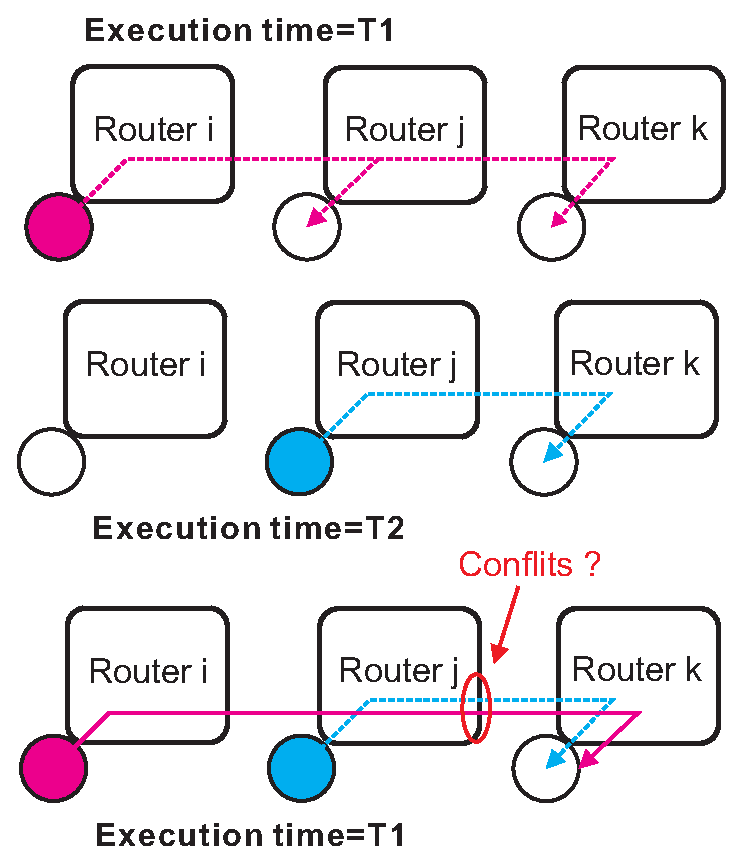
\includegraphics[width=0.6\columnwidth]{router.eps}
  \vskip -2mm
  \caption{An example of how a data dependency has an impact on traffic behaviors.}
  \label{fig:router}
  \vskip -8mm
\end{figure}
\subsubsection{Vision of the Model}
An application consists of different tasks and their interactions (i.e., inter-task data and non-data dependencies). To analyze the structure and dynamics of its tasks, one can represent the application using graphical models where tasks are represented as nodes and task interactions as edges. In spite of their wide use in validating the resource scheduling, task mapping, automatic parallelization as discussed in Section 2, their application to modeling the runtime application traffic behaviors is limited. For instance, communication task graphs (CTG) used in prior NoC studies are not able to capture dynamic data dependencies, i.e., when a data set is generated,  exchanged and how different data sets are related at runtime. Ignoring such dependencies might lead to biased network performance measurement. To give an intuition, we show a simple PE-based NoC example in which ignoring the data dependencies can lead to erroneous estimates of the NoC performance for an application of interest. \\
\indent Figure~\ref{fig:router} shows three routers $i, j$ and $k$ (each with a single input buffer) interfacing three processing elements (PEs) and exchanging data for calculating the average and variance of a time series stored in tile $i$. Let us assume PE $i$ sends this data to PEs $j$ and $k$. The results computed by PE $j$ will be reused by PE $k$, i.e., the average of the data set will be sent to PE $k$ for calculation of the variance, thus there is data dependency between these two tasks (i.e., calculation of average and variance). During execution, what really happens is that the packets issued by PE $j$ might never have conflicts with those injected by PE $i$ because the computation in PE $j$ usually takes more time than what it takes to move the data from PE $i$ to PE $k$. However, if we use a conventional CTG or even a trace-based benchmark that does not consider task dependencies, we might end up with erroneous network performance measurement. This happens when the link between Router $i$ and $j$ is heavily congested such that the packet injected by Router $i$ waits longer than the computation time of PE $j$. In such case, Router $j$ would still mistakenly inject the "results" as instructed by the collected trace even it has not received full data set from Router $i$, resulting in a unrealistic traffic pattern.\\
\indent To address these problems, we propose a dynamic graphical model learned at runtime not only for accurate characterization of the application but also practical use as realistic traffic generator. More precisely, we propose to model each task as a data generation system, which consists of: i) a timed finite state machine that governs its system state transition at runtime and ii) a data generation process that determines its communication patterns. By relating the input of the system to the system state transition that determines the output in a timed fashion, the proposed model is able to capture runtime inter-task dependencies and characterize the spatio-temporal patterns of the communication.
\subsubsection{Model Description}
%The keystone of the model is to set up an abstraction of \textit{task} to understand what it is and how it affects the communication. A intuitive description of a task given a specific application is a component that takes data from upstream tasks or user entries as input, performs an operation on those data, and generate a new set of data as output for tasks in the subsequent execution path and send them following a certain pattern, i.e., a specific distribution of data generation. Given a fixed task, a different set of data input might result in different set of output and the associated data generation process,  based on the state of task execution. Consequently, instead of modeling a task as a single node, we define the task as a data generation system with following formalism, \\
%so the system stata pathway matters ! 

The keystone of the model is to set up an abstraction of the application that is able to not only mathematically expressive in capturing the runtime application behaviors and its task structure, but also practically easy to be learned and used for realistic traffic generation. Towards this end, we follow the same idea to characterize a parallel program from a compiler perspective and define an application as a collection of tasks. Each task can be understood as a sequence of basic operations. Given a task, its execution might have i) data dependencies (i.e., it requires the output of other tasks) and/or ii) non-data dependencies (e.g., synchronization) on prior tasks. Once these dependencies are satisfied, the behaviors of tasks can be summarized as: i) processes its input (either from prior tasks or from user input), ii) generates a new set of data as output for tasks in the subsequent execution path and iii) exchanges them following a specific pattern (i.e., a specific distribution of data generation). Intuitively, a task can be abstracted as data generation system: it checks upon its input and transits its state from IDLE to READY as its dependencies on prior tasks are satisfied over time. If the system enters READY, it will operate on its input and map them to output over an execution time horizon. Otherwise, it will keep still and waiting for the receipt of all its input. To formally characterize it, we introduce the following definition:\\
\noindent \textbf{Definition 1:}\label{def:task} \textit{ An application task $\mathcal A(t)$ is a data generation system determined uniquely by a quadruple $(\mathcal M, \mathcal G(t), \mathcal T, \mathcal C)$  over time horizon $[t,t+\mathcal T]$. $\mathcal M$ is a timed finite state machine. \{$\mathcal G(t)$, $t\in \mathcal T$\} is a data generation process where $\mathcal G(t')$ denotes the number of data units generated over time interval [$t,t+t'$]. Function $\mathcal C$ maps a task $\mathcal A(t)$ to a set $\mathcal C(\mathcal A(t))$  containing all other prior tasks upon which the execution of $A(t)$ has dependencies. } \\
\indent An application task $\mathcal A(t)$ is defined over its execution horizon $\mathcal T$, i.e., its active time period. To run task $\mathcal A(t)$, all prior tasks in $\mathcal C(\mathcal A(t))$ have to be finished. To check upon whether such dependencies are met over time, $\mathcal A(t)$ maintains a timed state machine $\mathcal M$ to drive system state transition from IDLE to READY. Upon READY, the execution will be initiated to generate a new set of data that might be used for subsequent tasks. The data generation can be characterized by a process \{$\mathcal G(t)$, $t\in \mathcal T$\}. To detail the timed state machine $\mathcal M$, we formally introduce the following definition:\\
 \noindent \textbf{Definition 2:}\label{def:machine} \textit{ A timed finite state machine $\mathcal M$ is a sextuple $(\mathcal I,\mathcal S, s_{0}, \mathcal O,\mathcal F, \Omega$) where $\mathcal I,\mathcal S,$ and $\mathcal O $ are finite disjoint sets of inputs, states and outputs, respectively. $s_{0}$ is the initial state. $\mathcal F$ is the transition function $\mathcal F: 2^{\mathcal I} \times \mathcal S \times 2^{\mathcal T} \rightarrow \mathcal S$. $\Omega$ is the output function $\Omega: \mathcal S\times \mathcal T \rightarrow 2^{\mathcal O}\times 2^{\mathcal T}$.}\\
 \indent Of note, $\mathcal I$ and $\mathcal O$ are the input and output alphabet with finite symbols, respectively. The idea is to introduce these two sets to model the input and output of a task. $\mathcal I$ and $\mathcal O$ provide abstract description of different dependency types. In practice, we use a simple integer alphabet $\{0,1,2\}$ for both $\mathcal I$ and $\mathcal O$. The input is $"0"$ if no corresponding dependency is met. Otherwise, $"1"$ and $"2"$ denote data dependency or non-data dependency, i.e., synchronization requirement, is satisfied, respectively. We use the finite alphabet set to avoid any architecture-specific assumptions, e.g., type of data or width of channels, such that the model is self-contained and general without a specific machine model, which might limit the applicability of the formalism.\\
  \indent $\mathcal F$ is a \textit {timed} transition function that maps a vector of inputs $I(\mathcal A(t))=\{i_k|i_k \in \mathcal I\}$, the current state $s \in \mathcal S$ and a vector of time stamps \{$t_k$\} associated with $I(\mathcal A(t))$ to the next state.  We refer to $i_k \in I(\mathcal A(t))$ as an input channel and $|I|$ is the width of input channel. Each input channel  $i_k \in I(\mathcal A(t))$ is paired with a time stamp $t_k$ (denoted as $(i_k, t_k)$) which determines the earliest time that $i_k$ can be checked. We introduce this time stamp to consider the time cost of task execution and communication which will be later detailed in the discussion of output function $\Omega$. Each $i_k$ connects to an output of an upstream task on which the execution of task $\mathcal A(t)$ depends, thus $|I(\mathcal A(t))|=|\mathcal C(\mathcal A_{t})|$. The task dependency of $\mathcal A(t)$ on a prior task $\mathcal A'(t)$ is satisfied if and only if a letter $"1"$ or $"2"$ in $\mathcal I$ is received by input channel $i_k \in I(\mathcal A(t))$ and its associated time stamp $t_k$ is not greater than current time stamp $t$ when the transition condition is being checked, i.e., the causal constraint. In contrast to ordinary finite state machine, we introduce an extra \textit{temporal} dimension to guard the state transition such that the timing information of the application can be captured. Consequently, the transition function $\mathcal F$ would drive the system state into READY if and only if $i_k \neq 0$ and $t_k \leq t$, $\forall i_k  \in I(\mathcal A(t))$.\\
  \indent The output function $\Omega$ maps the timed current state $(s,t)$, where $s\in\mathcal S$ and $t \in \mathcal T$,  to a vector of output $O(\mathcal A(t))=\{o_k|o_k \in \mathcal O\}$, guarded by an array of time stamps \{$t+\delta_k$\}. Similarly, we define $o_k \in O(\mathcal A(t))$ as an output channel.  $\delta_k$ denotes the \textit{delay} of output channel $o_k$ caused by the execution of the task on the input data set $I(\mathcal A(t))$ and the data generation process, i.e., communicate data over a certain period of time, is equal to $\delta_{k,e}+\delta_{k,c}$, the execution delay and communication delay, respectively. Of note, $\delta_{k,e}$ replies on mapping function from the task to a specific processing entity (e.g., a dedicated PE or a processor), i.e., the delay is decided by how "fast" the task can be processed. In the model, we have no assumption on mapping function or processing entity, hence enhancing the expressivity of the model. $\delta_{k,c}$ is the \textit{span} of the data generation process which is described by $\mathcal \{\mathcal G(t), t\in \mathcal T\}$. Given a specific task, the data generation process could be arbitrarily complicated whereas it is still possible to find a \textit{best-fit} stochastic process model that best characterize its behaviors. For instance, the process could be memory-less (e.g., Poisson process), long-range memory (e.g., self-similar or fractal process) or a general $\alpha$-stable process.\\
  \indent Connecting Definition~1 and 2, we have constructed the backbone of the model for NoC applications. Compared to the conventional definition of task in context of parallel program analysis, we view each task as a data generation process whose behaviors are governed by a timed state machine $\mathcal M$ and data generation process $\mathcal G(t)$ given the execution time horizon $\mathcal T$. Its dependencies are characterized by $\mathcal C(\mathcal A(t))$.  Given a collection of tasks $A=\{\mathcal A_i(t)\}$, we are able to construct a graphical model $\mathcal B(t)=(A,E,t)$ where each vertex $a_i$ corresponds to an application task $\mathcal A_i(t)$ and each directed edge $e_{i,j}$ exists if and only if task $a_i$ has, either data or non-data, dependency on task $a_j$. Formally, we have the following definition,\\
\noindent \textbf{Definition 3:}\label{def:app} \textit{ A NoC application $\mathcal B(t)=(A,E,t;\mathcal T)$ over its execution time horizon [$t$,$t+\mathcal T$] is a \textbf{dynamical directed graph} where each vertex $a_{i} \in A$ is an application task $\mathcal A_i(t)$ and edge $e_{i,j} \in E$ if and only if $\mathcal A_{j}(t) \in \mathcal C(\mathcal A_{i}(t))$.}\\
\indent In contrast to previous graphical model for application traffic, the proposed model not only translates the spatial dependencies into geometric characteristics of the graph (i.e., nodes, edges and their connection pattern), but also introduces a detailed description for tasks that are able to preserve the temporal dependencies. In the following discussion, we will present a traffic synthesis technique based on the proposed model to address the problem \textbf{P$_2$)}.
\subsection{Benchmark Workloads synthesis}
The large-scale benchmark synthesis problem can be stated as follows: \textit{How can the traffic be generated for a given size and the application profiled by the proposed model $\mathcal B(t)=(A,E,t;\mathcal T)$ such that traffic characteristics of the real application are preserved ?}. Thus, our objective is to build a traffic generator for NoC evaluation without interfacing it with a full-system simulator such that, the target NoC is identically stressed but requires less simulation time. \\
\indent To formally define the problem, let $A$ be the universal set of tasks involved in $\mathcal B(t)$. Assume $|A|=n$, let $S(t)$ be the $n$-dimensional state vector of $\mathcal B(t)$ such that $S(t)=[s_0(t),s_1(t),\dots,s_{n-1}(t)]^{T}$. We define the vector sequence $E_0=$<$S(0),S(\Delta t),S(2\Delta t),...$ $S(\mathcal T)$> as the \textit{recorded states of tasks during application execution on target architecture over finite horizon $[0,\mathcal T]$}. In other words, $E_{0}$ is the task state transition trace recorded from the execution of the real application. We define $E(\mathcal B(t))$ = < $S(0)$, $S(\Delta t)$, $S(2\Delta t)$$,...,$ $S(\mathcal T)$> as \textit{an execution of benchmark $\mathcal B(t)$ over a finite horizon $[0,\mathcal T]$} where $\Delta t$ is time step of interested length, i.e., the cycle of simulation clock. Intuitively, $E(\mathcal B(t))$ is the simulated system state transition trace. Since it is observed that the output of each task is \textit{uniquely} decided by the system state $s$ and the time stamp $t$ through the mapping relation $\Omega$ for each task $\mathcal A_{i}(t)$ (see Definition 2). Therefore, the system state transition trace determines the traffic characteristics of the application. As a result, given an execution horizon $\mathcal T$, ideally, the simulated system state transition trace  $E(\mathcal B(t)) $ should be equal to the recorded state trace $E_0$. Formally, we can formulate the benchmark synthesis problem  as :\\\\
\noindent\textbf{NoC benchmark synthesis problem :} \\
\textbf{Given} an application profiled by $\mathcal B(t)$, a target architecture, execution time $\mathcal T$ and the recorded application state transition trace $E_{0}$ \\
\textbf{Determine} the initial state $s_0$, output function $\Omega$ and data generation process $\mathcal G(t)$ for each task $\mathcal A_{i}(t)$ to obtain an execution $E(\mathcal B(t))$ of $\mathcal B(t)$ to minimize its deviation from the recorded trace: 
\begin{equation}\label{eq:prb1}
   \min\limits_{s_0,\Omega,\mathcal G(t)} ||E(\mathcal B(t))-E_0||^2
\end{equation}
Equation~\ref{eq:prb1} shows the proposed model enables us to provide a way to quantify the similarity of the characteristics between the synthesized traffic and the real application traffic by measuring the norm of deviation of state transition trace in both cases. \\
\indent To solve this problem, it should be first noted that the source of difficulty in minimizing~(\ref{eq:prb1}) resides  both in accurately identifying the task structures, i.e., tasks and their runtime inter-dependencies, and capturing its communication patterns (e.g.,g memory access events), i.e., learning the data generation process $\mathcal G(t)$. We thus propose a synthesis framework based on runtime architecture-independent model learning. Figure \ref{fig:OVERVIEW} shows the overview of the proposed benchmark synthesis framework. The overall framework could be understood as a two-stage process where i) an \textit{architecture-independent} application profiling and model learning stage is set up for analysis of runtime application task graph and construction of the NoC application model $\mathcal B(t)$ upon which ii) a subsequent benchmark generating stage is built to introduce realistic variation to the generated traffic model for extrapolated traffic synthesis given a \textit{target} architecture. It should be noted that, instead of extracting static task graphs, we define NoC application model $\mathcal B(t)$ in Section 3.2.2 as a dynamical graph that can only be learned during the execution of the program. This is because the statically extracted task graph is not a sufficient representative of the applications with unknown tasks and their spatio-temporal inter-task dependencies prior to execution of them.\\
\indent Specifically, we have modified the Contech compiler~\cite{railing2015contech} that is based on the LLVM compiler framework~\cite{lattner2004llvm} with OpenMP support that provides the ability to observe and manipulate the intermediate representation of a program. Following Contech compiler, the adopted profiling methodology is two-layered. The first layer is used to take the source code of the application as input and translate it into instrumented LLVM intermediate representation(IR).  The compiler in the \textbf{first layer} will run a function-by-function check to identify the basic blocks (e.g., basic actions or predefine functions) and insert inlined codes into target ISA assembly to collect the properties of memory access events, i.e., address, size, type and timing information \textit{during the execution time of the application}. To capture the inter-task dependencies, the synchronizing actions are identified through analyzing the LLVM IR or the name of the function invoked. The address of the action, the order of the action with respect to other synchronization actions on this address and time stamps from before/after the action will be recorded in a local buffer for each thread. Eventually, a global event list will be generated where events from the same thread are stored in the \textit{event list in program order} rather than the micro-architectural order from out-of-order processors or memory consistency, thus avoiding specific architectural assumptions. \\
\indent \textbf{The second layer} takes the extracted event list to infer the application model $\mathcal B(t)$. Each task accumulates a list of basic block IDs and memory accesses from the event list until a synchronizing action is encountered. Then all previous blocks are assumed to be in the same \textit{context} and merged into a single task $\mathcal A_{i}$. The task dependencies between other synchronizing actions are checked such that for each $A_{i} \in \mathcal B(t)$, we are able to determine the input channel $\mathcal I(\mathcal A_{i})$ (or output channel, equivalently) upon finishing processing all basic blocks in the event list. Alternatively stated, we are capable of construction of node $\mathcal A_{i}$ and edge $e_{i,j}$ of all choice of $i$ and $j$ for $\mathcal B(t)$ given the event list collected by the LLVM compiler with instrumentation at execution time. This constitutes the topology, i.e., the structural features, of the proposed graphical model. Recall that we define application task $A_{i}$ as a quadruple \{$\mathcal M,\mathcal G(t),\mathcal T, \mathcal C$\} where function $\mathcal C(A_{i})$ denotes the subset of tasks dependent on $\mathcal A_{i}$. By identifying tasks and their dependencies, we have learned also the function $\mathcal C$.\\
\indent To practically use the graphical model to generate traffic aligned with realistic application behaviors, we should derive finite state machine $\mathcal M$ and data generation process $\mathcal G(t)$ also from the collected trace in the first layer. We define each input channel of a task to correspond to the dependency on a upstream task. The state transits as any of its dependencies on prior tasks are met, i.e., either data or synchronizing dependencies are satisfied. The date generation process $\mathcal G(t)$ is initiated once the state machine $\mathcal M$ enters the end state where all dependencies are satisfied. Recall that we have recorded all memory access events by running the instrumented program. All memory access events, when mapped to a NoC-based architecture, translate to data injection events. Combined with time stamp of the memory accesses recorded, it is possible to either i) directly use the trace or ii) fit a stochastic process $\mathcal G(t)$ for data injection of each task $\mathcal A_{i}$. Together with execution horizon $\mathcal T$ which we use to run the program, we have learned the application traffic model $\mathcal B(t)$.\\
 \indent It should be noted that fitting a stochastic process $\mathcal G(t)$ to the recorded data generation process could be arbitrarily difficult as it might not be aligned with a known stochastic process or changes quickly over time such that we do not have sufficient data for estimation of the distribution parameters. Otherwise, we can fit a stochastic model to \{$\mathcal G(t),t$\} to further reduce the complexity of the model. As a case study, we assume $\mathcal G(t)$ follows a Poisson distribution such that for output channel $o_k$: 
\begin{equation}\label{eq:poisson2}
   P\{\mathcal G(\Delta t)=k\}=\frac{\lambda \Delta t^{k}}{k!}e^{-\lambda \Delta t}
\end{equation}
$\lambda$ is the strength of Poisson flow. Given the size of data to be generated as $L$, the statistical average of $\delta_{k,c}$ is given by,
\begin{equation}\label{eq:solu}
   \textbf{E}[\delta_{k,c}]=\frac{L}{\textbf{E}[\mathcal G(\Delta t)]}\Delta t 
\end{equation}
Since $\textbf{E}[\delta_{k,c}]$ is an unbiased estimate of $\delta_{k,c}$, we use $\textbf{E}[\delta_{k,c}]$ to replace $\delta_{k,c}$. Of note, the assumption of Poisson distribution is helpful to give a case study whereas Equation~(\ref{eq:solu}) can be applied to other processes.\\
\indent Given the constructed model $\mathcal B(t)$, a follow-up question is how can we make changes to the graphical model such that i) we can simulate the runtime variations of the traffic (i.e., Problem \textbf{P}$_3$), and ii) how can we scale it to test different NoCs while preserving its spatial-temporal characteristics of traffic (i.e., Problem \textbf{P}$_2$). Next, we address these problems by proposing a network generation algorithm based on complex network theory. 
\section{Evolvable Benchmark Synthesis}
\subsection{Overview}
Given an application described by the proposed model $\mathcal B(t)$, it is desirable to generate an array of benchmarks that are diverse in scales but ``similar" in spatial and temporal behaviors as the $\mathcal B(t)$. As we discussed in Section 3, the spatial dependencies are encoded by the structural characteristics of $\mathcal B(t)$ while the temporal dependencies are embedded in structure of the task (i.e., the timed finite state machine $\mathcal M$ and the data generation process $\mathcal G(t)$).  Therefore, an efficient way to preserve such dependencies when editing the graph is to keep \textit{key structural features} of the model at \textit{proper scales}. For example, if we look at the graphical model at the highest scale, we will observe a single node. Then we replicate this single node and go back to the original scale. We will expect a very similar graph as the original one but doubled in size. Following the same idea, we can preserve any structure in the graph as long as we replicate a coarsened node at a proper scale. More precisely, we propose a scaling algorithm based on complex network generation that produces graphs that are similar to $\mathcal B(t)$. 
\subsection{Measuring the Graph Similarity}
\begin{figure}%[htb]
  \centering
  % Requires \usepackage{graphicx}
 % \epsfig{file=t_calc.eps}
  \includegraphics[width=1\columnwidth]{assort.eps}
  \vskip -2mm
  \caption{Example graphs visualize assortativity, betweenness and clustering }
  \label{fig:assort}
  \vskip -3mm
\end{figure}
\begin{figure}[t]
  \centering
  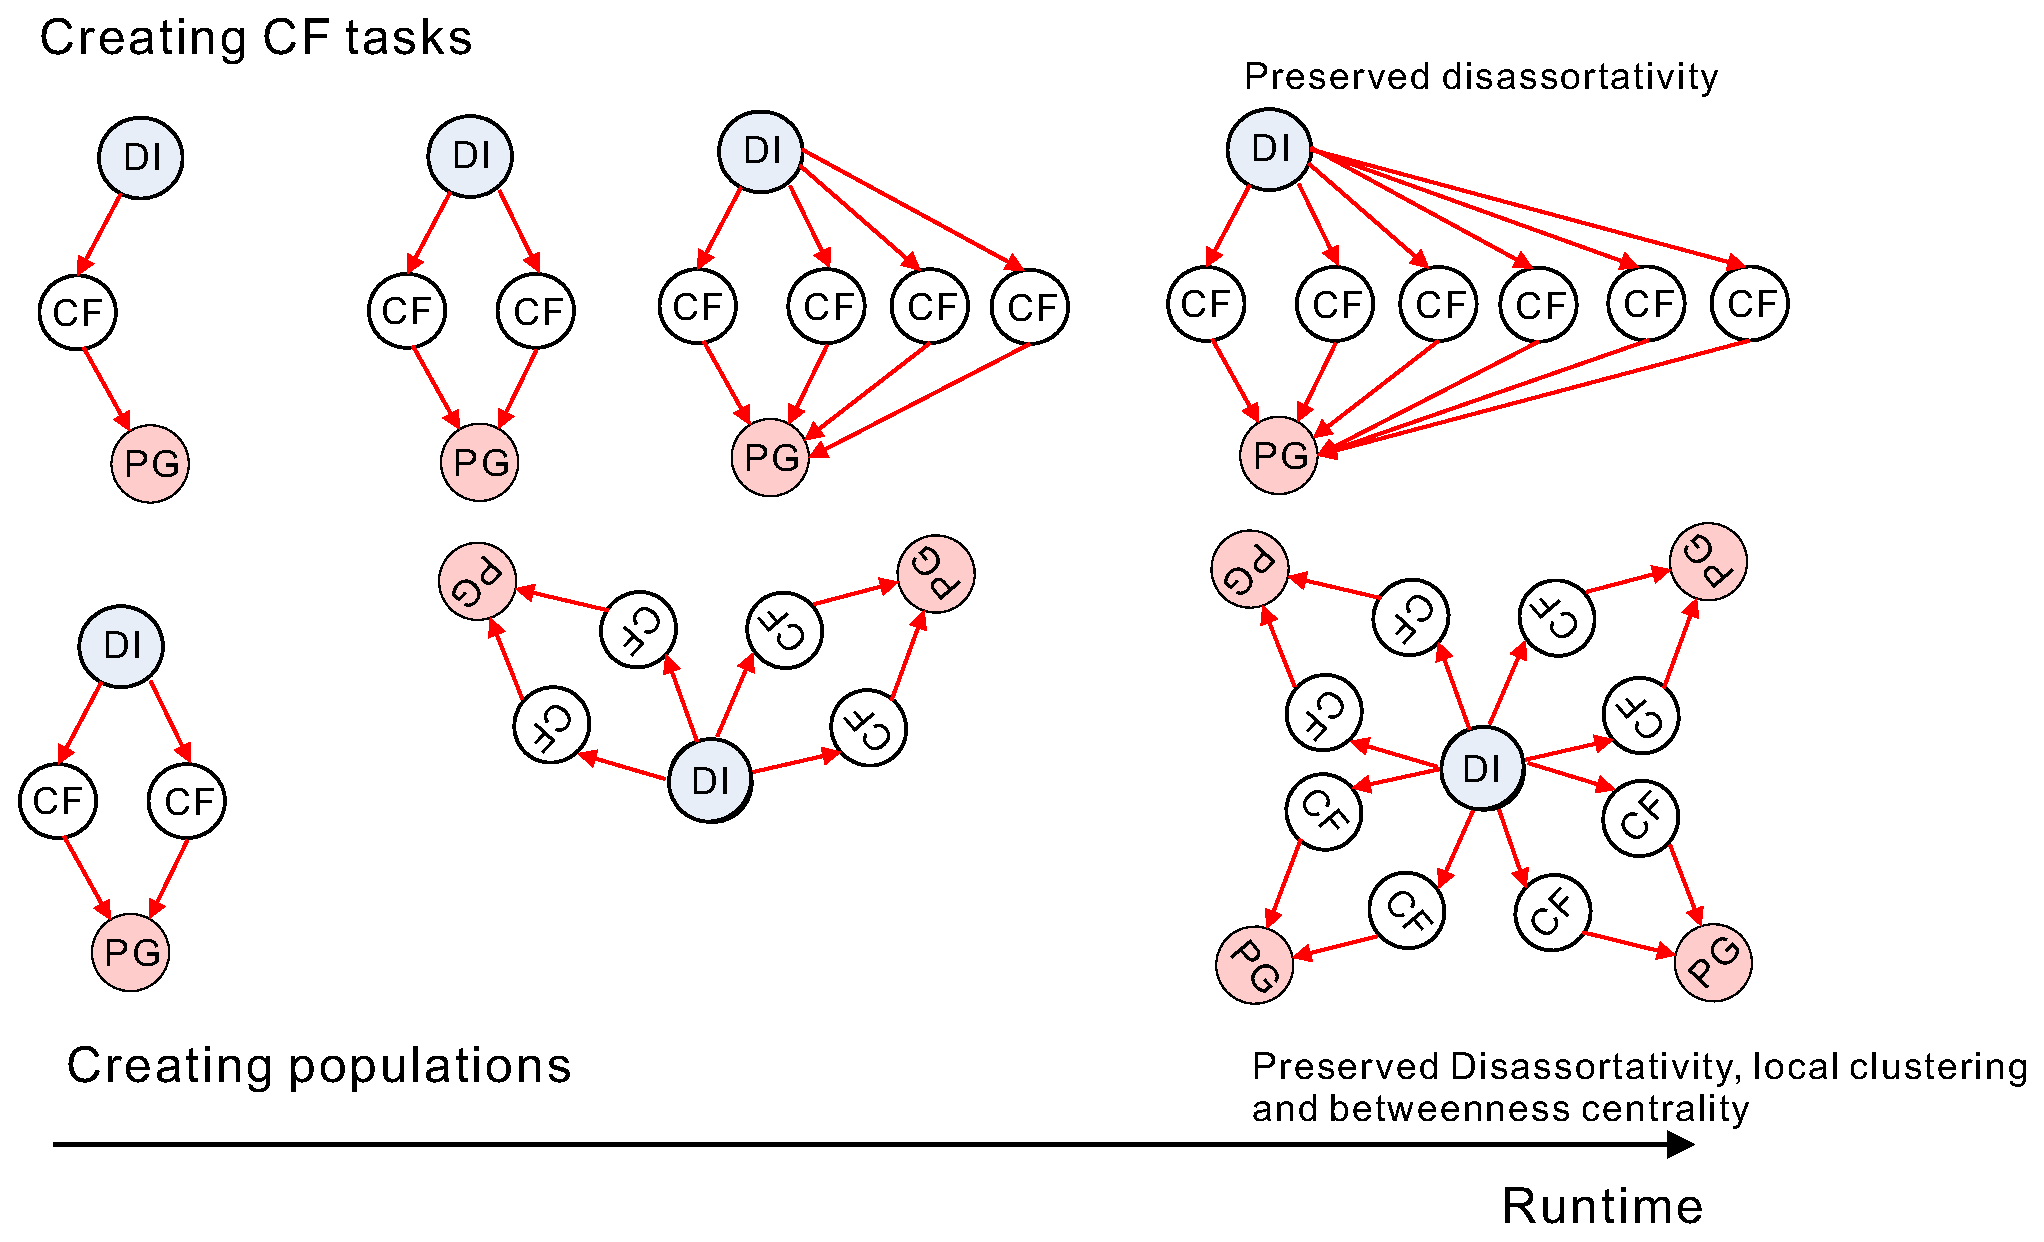
\includegraphics[width=1\columnwidth]{evl.eps}
  \vskip -2mm
  \caption{The evolution of genetic algorithm at runtime.}
  \label{fig:fig_evl}
  \vskip -5mm
\end{figure}
To measure the similarity between graphs of various sizes, we introduce a set of structural metrics $M=\{\alpha, \beta, \gamma, D_{avg}, P_{avg}\}$ which are well used for comparing graphs. The average node degree $D_{avg}$ shows the local interconnection strength. The average path distance $P_{avg}$ shows the average distance between all possible pairs of nodes in the graph.\\
\indent We denote $\alpha$ as the \textbf{assortativity} metric which measures the tendencies of nodes to connect with other nodes that have similar degrees as shown in Figure~\ref{fig:assort}. For directed graphs, the \textit{in} and \textit{out}-assortativity are measured, respectively. In general, $\alpha$ lies between $-ˆ’1$ and $1$. When $\alpha = 1$, the network is said to have perfect assortative mixing patterns, when $\alpha$ = 0 the network is non-assortative, while at $\alpha = -ˆ’1$ the network is completely disassortative. The \textbf{clustering coefficient} $\gamma$ is a measure of the degree to which nodes in a graph tend to cluster together. The \textbf{betweenness centrality} $\beta$ is an indicator of a node's centrality in a network. It is equal to the number of shortest paths from all vertices to all others that pass through that node. Betweenness has important implications for the proposed graphical model. To give an intuition, we visualize these metrics in Figure~\ref{fig:assort} using example graphs.\\
\indent To understand the physical meaning of the metrics and motivate their link to the task structures in a realistic setting, we present a case study where we run the multi-threaded coarse grain hierarchical parallel genetic algorithm (HPGA)  and show variations in task structure over time in Figure \ref{fig:fig_evl}. The sequential version of HPGA has very simple  task structure consisting of three basic blocks: i) Distribution of individuals (DI), i.e., candidate solutions; ii) Calculation of fitness (CF); iii) Produce the new generation (PG) based on fitness. In the example, the host is able to create new CF tasks and populations, i.e., a pool of candidate solutions, to parallelize the execution. Over the execution time, the task structure has been through variations whereas preserving several important structural features: i) The disassortativity of the graph is respected and preserved, i.e., nodes of high degree tend to connect to nodes with low degree. The task graph of HPGA is strongly disassortative suggesting the existence of global synchronization nodes. ii) The majority of nodes remains less clustered which indicate the source of potential parallelism; iii) The DI task preserves its high betweenness centrality as multiple populations and corresponding CF and PG tasks being created, which suggests DI as a synchronization node.\\
\indent  Even though the example is just a case study with very simple task structure, yet we can make the following observations: i) The structural feature analysis on the extracted application task graph can help us identify the critical tasks such as synchronization node and potential parallelism. ii) By preserving key structural features like assortativity (not necessarily the absolute value of the metrics), we might be able to introduce realistic variations to the original task graph especially when we have no prior knowledge on how the real application changes over time. Based on these observation, we next present our benchmark scaling algorithm.
\subsection{A Complex Network-inspired Benchmark Scaling}
\begin{algorithm}[tb]         %Ëã·¨µÄ¿ªÊ¼
\caption{Benchmark scaling algorithm  \textbf{Gen}($\mathcal B(t)$)}             %Ëã·¨µÄ±êÌâ
\label{alg:main}                  %¸øËã·¨Ò»¸ö±êÇ©£¬ÕâÑù·½±ãÔÚÎÄÖжÔËã·¨µÄÒýÓÃ
\begin{algorithmic}[1]                %²»Öª[1]ÊǸÉÂïµÄ£¿
\REQUIRE ~~\\

    Graph seed $\mathcal B(t)$; Selected metric set $M'\in M$; 
    Downscaling function $\Gamma$; Upscaling function $\Gamma^{-1}$; Editing function $\Pi$; Expected size of graph $N$                

\ENSURE ~~\\                           %Ëã·¨µÄÊä³ö£ºOutput
    A set of accepted graphs  \textbf{$\mathcal B'(t)$}
\STATE i=0;
\IF{Sanity\_check$(\mathcal B(t))$==false}
\STATE Return $\mathcal B(t)$
\ELSE
\STATE $\mathcal B'(t)$=$\Gamma(\mathcal B(t))$
\STATE $\mathcal B'(t)$=\textbf{Gen}($\mathcal B'(t)$)
\WHILE{$ |V'(t)|<N $ and $||M'(\mathcal B(t))-M'(\mathcal B'(t))||_{2} > \Delta$}
\STATE $\mathcal B(t)_{scaled}$=$\Gamma^{-1}(\mathcal B'(t))$
\STATE $\mathcal B'(t)$=$\Pi(\mathcal B(t)_{scaled})$
\ENDWHILE
\STATE Return $\mathcal B'(t)$
\ENDIF
\end{algorithmic}
\end{algorithm}
Let us define the editing function as $\mathcal E: V\times E \rightarrow V\times  E$ and $M(\mathcal B(t))$ as the similarity vector under above-mentioned metrics $M$. The problem to generate evolvable benchmarks can be formally stated as:\\\\
\noindent\textbf{NoC benchmark scaling problem} \\
 \textbf{Given} an application profiled by $\mathcal B(t)$ and the metrics of interest $M'\subset M$.\\
 \textbf{Determine} a sequence of editing function $\mathcal E=$ <$\mathcal E_0,...,\mathcal E_{n-1}$> such that
\begin{equation}\label{eq:prb_evl}
 \min\limits_{\mathcal E_0,...,\mathcal E_{n-1}} ||M'(\mathcal B(t))-M'(\mathcal E(\mathcal B(t)))||^2
\end{equation}
\textbf{Subject to:} 
\begin{equation}\label{eq:prb_SUB}
|V'(t)|\geq N, V'(t) \in \mathcal E(\mathcal B(t))
\end{equation}
Starting with a $\mathcal B(t)$ as seed, we need to determine a series of editing functions applied to $\mathcal B(t)$ to generate $\mathcal B'(t)$ such that a subset of structural features $M'$ are preserved. \\
\noindent \textbf{Lemma 1:}\label{def:causal}
\textit{The problem described by~\eqref{eq:prb_evl} is NP-hard}.\\
\textit{Proof:} The proof follows by noticing that the calculation of the average path of a graph requires finding all the paths in a graph. Thus the problem solution contains the solution to  the longest path problem, which is NP-hard. Because the problem in~\eqref{eq:prb_evl} contains (as subclass of problems) one that is NP-hard, it follows that \eqref{eq:prb_evl} is also NP-hard.\\
\begin{figure}%[htb]
  \centering
  % Requires \usepackage{graphicx}
 % \epsfig{file=t_calc.eps}
  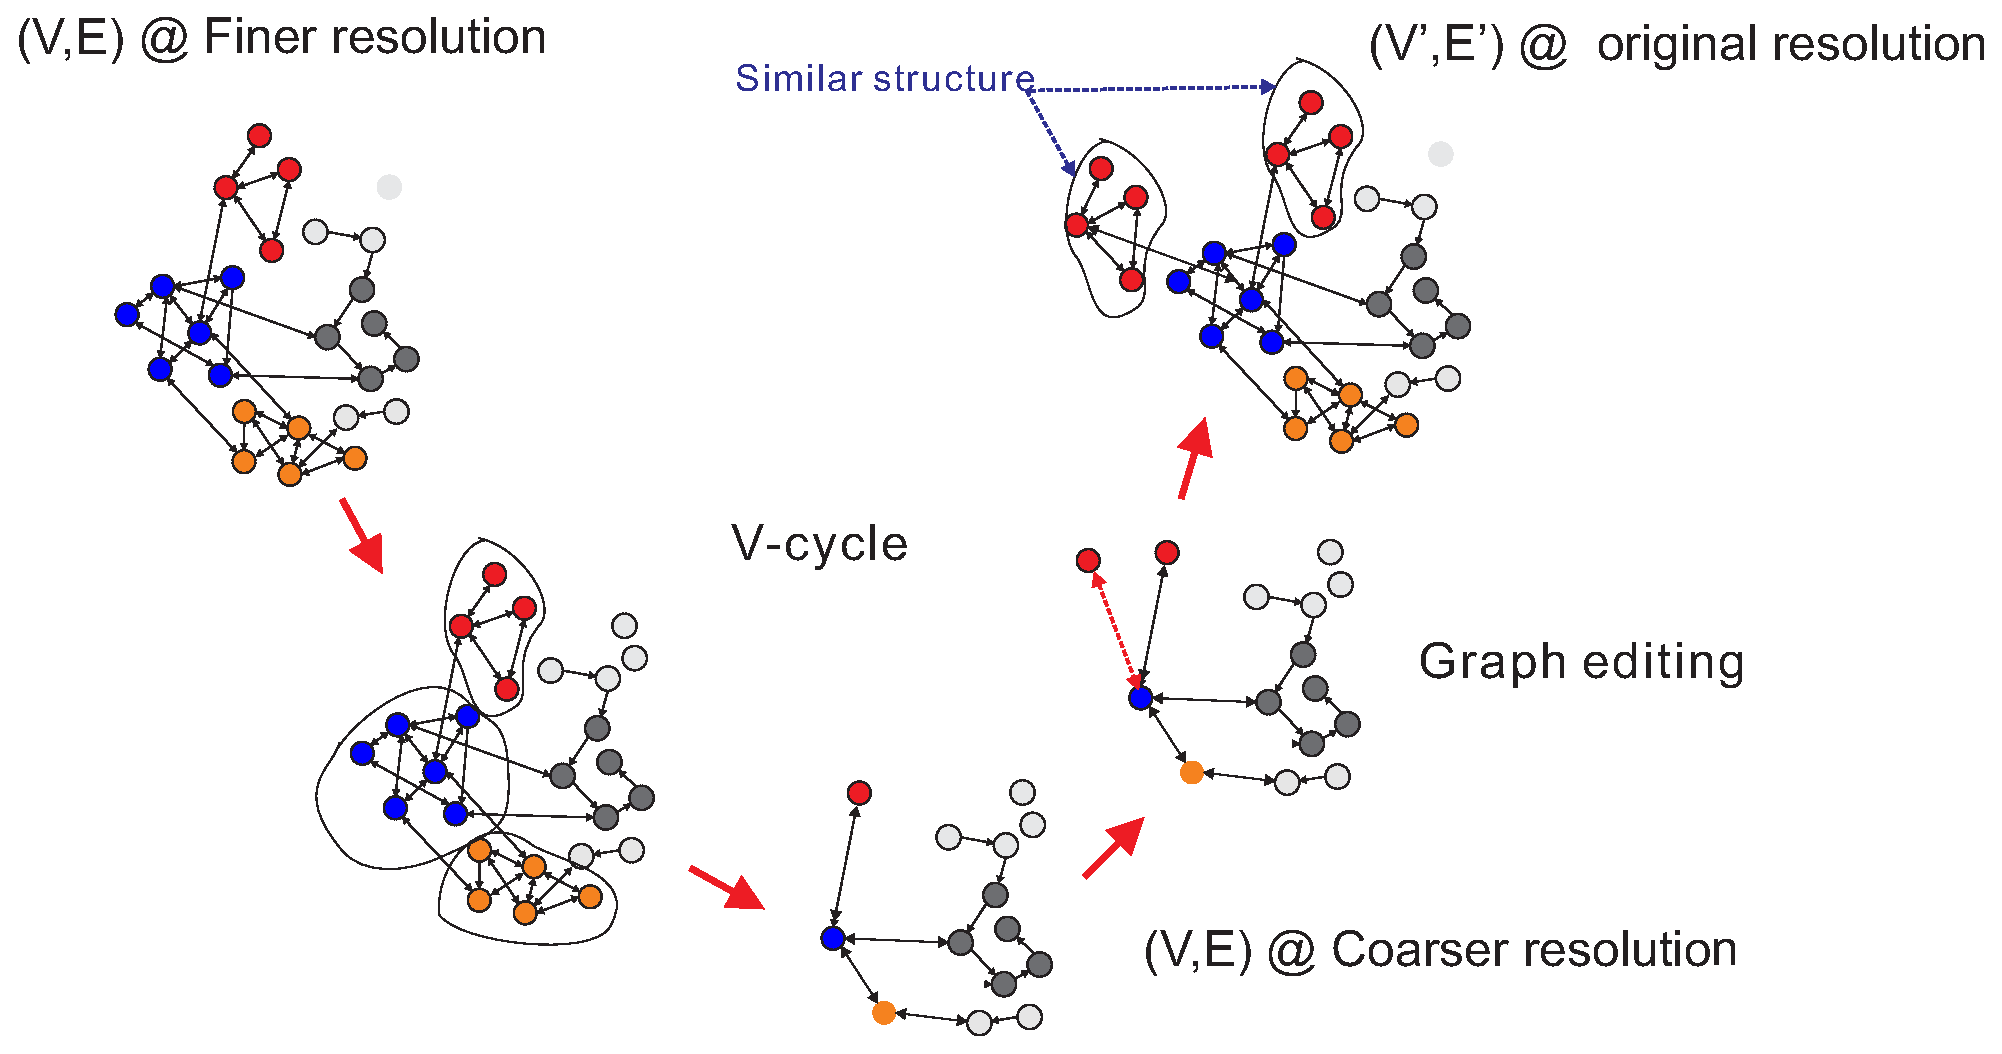
\includegraphics[width=1\columnwidth]{V.eps}
  \caption{The overview of benchmark scaling algorithm. The procedure follows a V-cycle of coarsening and refining operations. By preserving nodes under proper scales, it is able to protect the  structural features of interest.}
  \label{fig:V}
  \vskip -5mm
\end{figure}
\indent Therefore, we propose a heuristic to solve this problem, which is inspired by the complex network generation and multiscale theory applied to solve combinatorial optimization problem in \cite{ron2011relaxation}. Alg. \ref{alg:main} shows the overall procedure of proposed algorithm. The proposed algorithm is a V-cycle scheme that solves the problem described in~\eqref{eq:prb_evl} using coarsening and refining iterations at multiple scales as shown in Figure~\ref{fig:V}. Our proposed algorithm starts from a seed application profiled by graph $\mathcal B(t)$ and recursively change the graph into greater scales (i.e. upscaling) until a sanity check is violated. The sanity check will control how deep the V-cycle would go by setting a lower bound for both number of nodes and edges remained. Once violated, the upscaling stops. Then an array of downscaling functions are applied to project the graph with ``coarser details" to a graph of a finer resolution. After the graph is downscaled,  a series of editing functions, i.e., node replication, insertion or deletion, are performed. To scale the benchmark while preserving the structural characteristics of the original graph, only node replication is considered. In other cases like simulation of application variation, there is no restriction on editing operations. 
\section{Experimental Results}

\noindent\textbf{Experimental setup}: To validate our mathematical framework for benchmark generation and scaling that preserve structural features of the extracted task graph, we consider three graph-based application traffic benchmarks, \textit{blackscholes, canneal and freqmine} from Parsec $2.1$.  We present two sets of experiments to validate the proposed application traffic model and NoC benchmark synthesis algorithms. \\
\indent In the first set of experiments, we compare i) the packet injection patterns and ii) average latency of the network during the execution of the region of interest (ROI), i.e., parallel phase, from a full-system simulation,  and those on a dedicated cycle-accurate NoC simulator driven by the traffic generated by the proposed model. We learn the model $\mathcal B(i)$ by instrumenting the applications and collecting execution trace. The full-system simulation is performed by Gem5 simulator  on 32- and 64-core in-order 2 GHz Alpha ISA processor running over a Linux kernel of version 2.6.27 which is patched for supporting 4-64 Alpha cores. The NoC interfaced with the processors is following the Garnet network model with mesh topology under deterministic dimension-order routing (DOR). The flit size is set as 8 bytes. Each input port has 4 virtual channels and the depth of each virtual channel is 4-flit. The dedicated NoC simulator is a cycle-accurate simulator written in C++ with settings that are identical to those used in full-system simulation.\\
\begin{figure}%[htb]
  \centering
  % Requires \usepackage{graphicx}
 % \epsfig{file=t_calc.eps}
  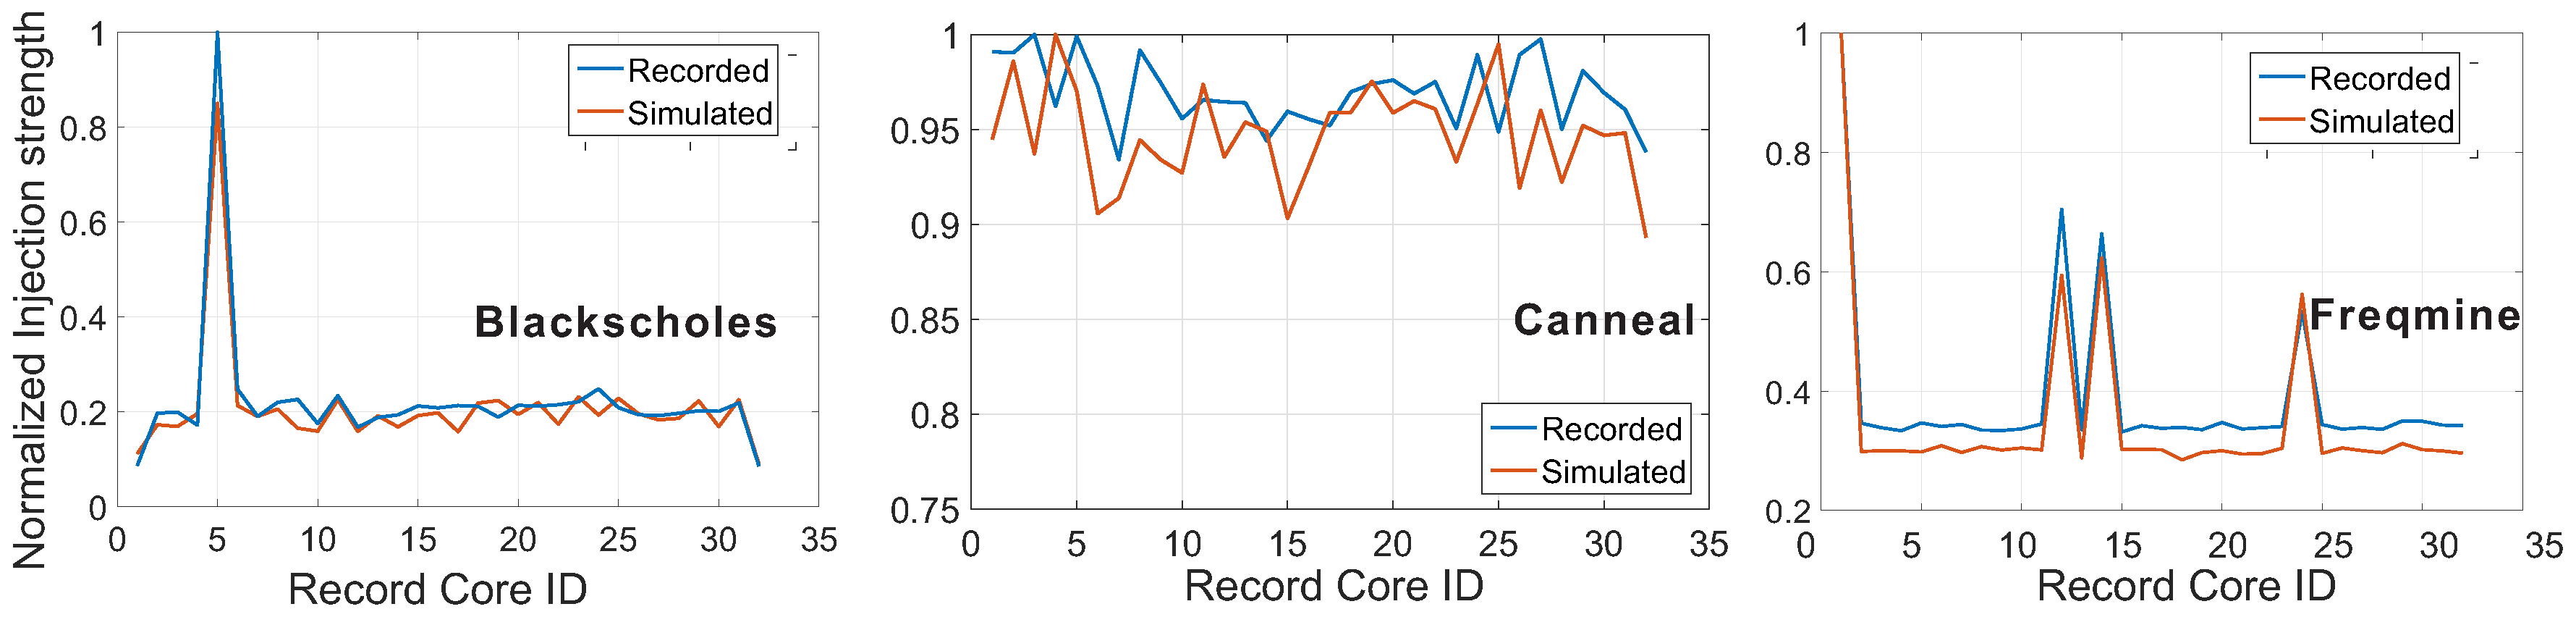
\includegraphics[width=1\columnwidth]{norm.eps}
  \vskip -2mm
  \caption{Measuring the distribution of injection strength over different processors under three application benchmarks, \textit{blackscholes, canneal and freqmine}, using both full-system simulation and synthesized traffic workloads based on the proposed model during ROI. The injection strength is calculated as the injection rate of a processor averaged over the execution time. In all three cases, the synthetic traffic workloads stress the target NoC to exhibit close injection distributions.}
  \label{fig:traffic_sim}
  \vskip -5mm
\end{figure}
\begin{figure}[ht]
  \centering
  % Requires \usepackage{graphicx}
 % \epsfig{file=t_calc.eps}
  \includegraphics[width=0.8\columnwidth]{latency.pdf}
  \vskip -3mm
  \caption{Comparison of average latency}
  \label{fig:lat}
  \vskip -5mm
\end{figure}
We first report three experiments performed under the full-system simulations using Gem5 on a 32-core system and the NoC stress test using a cycle-accurate C++ NoC simulator. To measure the goodness-of-fit of traffic behaviors using the synthetic traffic against those under the full-system simulation, i.e., whether the network communication exhibits close patterns under two workloads, we choose to measure the distribution of average injection strength during ROI over all 32 cores considered.  The average injection strength is calculated by averaging the total number of packets generated by the lapsed time. The results are reported in Figure~\ref{fig:traffic_sim} and normalized by the maximum injection strength of both cases. It is observed that the obtained distributions of injection strength under the synthesized NoC traffic are consistent with those measured during the full-system simulation in all three benchmarks. It should be noted that the injection strength distribution is contributed by all runtime communication and computation events that are either producing or consuming data. These events are inter-coupled via the task dependencies embedded in the execution path of the application.  Without the incorporation of such dependencies in the synthesized traffic, it is difficult to have close fitting to the real traffic behaviors that are usually identified through full-system simulation. In addition to injection strength distribution, we have also measured the average network latency for networks of different size driven by the full-system simulation trace or the generated traffic by the proposed model. The results are reported in Figure~\ref{fig:lat}. Under different network settings, the NoC simulation driven by the proposed model demonstrates consistently  close latency performance compared to that measured under full-system simulation with an error mean of $\%1.2$ and $\%2.1$ for 32-core and 64-core simulation, respectively.\\
\begin{figure}[tb]
  \centering
  % Requires \usepackage{graphicx}
 % \epsfig{file=t_calc.eps}
  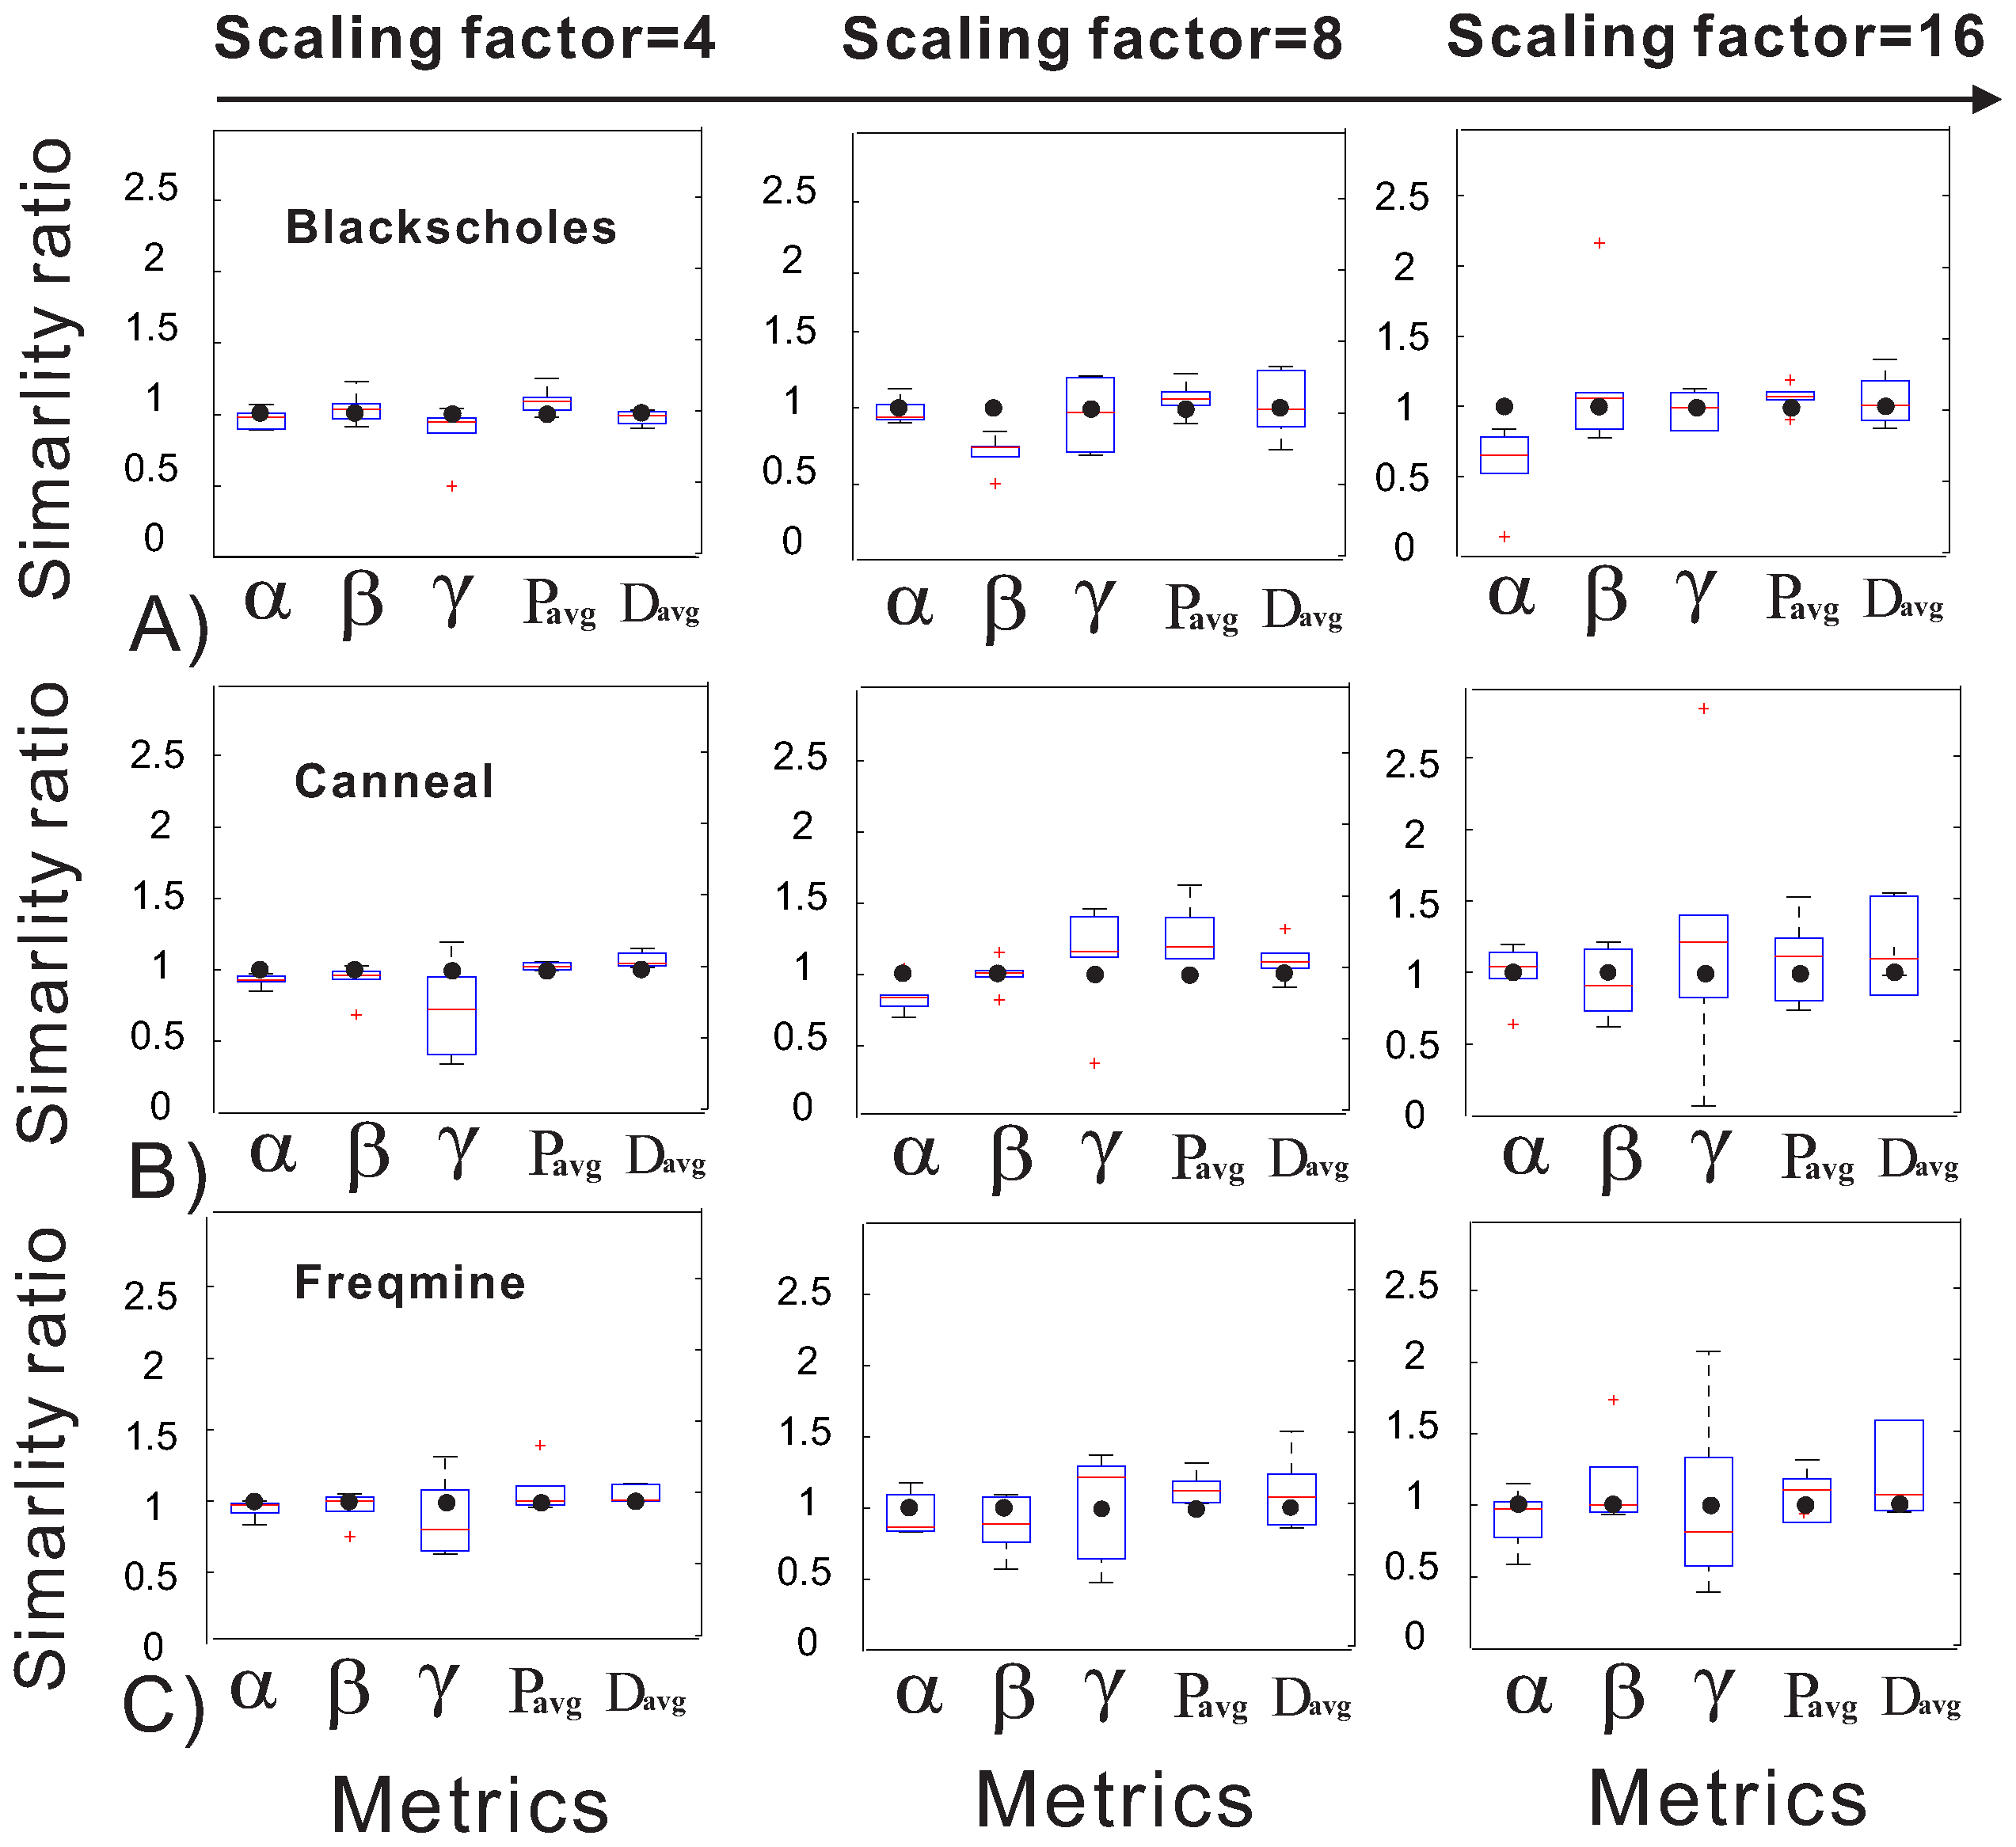
\includegraphics[width=0.8\columnwidth]{str_2.eps}
  \vskip -2mm
  \caption{Measuring structural similarities of graphical models scaled by a factor$= 4,8$ and $16$.}
  \label{fig:stru_sim}
  \vskip -7.5mm
\end{figure}
\indent In the second set of experiments, we would like to check whether the proposed model is able to scale up the application model constructed to an expected scale, meanwhile introducing minimized deviation in the set of interested structural metrics (see Section 4.2). To motivate the  protection of the structural features in a graphical model, not only the proposed model, but in general cases, we should be aware the following fact:  as we mentioned in the previous discussion, the structural characteristics of most of application graphical models, are naturally encoding the spatial dependencies via construction of their geometric structures, i.e., connection of nodes via edges. Actually, prior research efforts in parallelization of algorithms largely rely on the analysis of such structural features and their implications. The change in such structures has significant influence on the execution of the application. Obviously, scaling a graphical model that is able to be used for traffic synthesis is a shortcut to efficiently obtain an array of benchmarks. However, editing the model  arbitrarily might invalidate its applicability to traffic synthesis due to the loss of fidelity. Therefore, we propose the NoC benchmark scaling algorithm based on a complex network theory to obtain new models with expected scales, meanwhile respecting its original structural characteristics. \\
\indent We first constructed the model based on the collected application trace during the ROI phase for all three applications. Then, we use the models as seeds to perform the proposed algorithm. New models are generated with different sets of expected network sizes, i.e., scaling factor$=4, 8$ and $16$. We measured similarity under a set of metrics. The results are reported in Figure~\ref{fig:stru_sim}. For each scaling factor, the measurement is averaged over 100 iterations. Several key observations can be made from the results: i) The proposed algorithm maintains a low level of deviation on average across the set of metrics considered. For a scaling factor of 2, all three graphs stay quite structurally consistent with the original graph. ii) As the scaling factor increases, the average deviation increases due to the structural modification introduced randomly during the refining process. The refining process in the proposed algorithm will randomly connect the newly added node, replicated or randomly introduced, to a existing node in the graph. As the scaling factor goes up, the graph might undergo increased levels of coarsening and refining process, i.e., a "deep-V" process, which boosts the chance of modifications to the graph introduced randomly during the process. Overall, the proposed model can reliably scale the benchmark by at least a factor of 8 and preserving some set of metrics even with a factor of 16.
\section{Summary}
In this work, we have proposed a mathematical framework to synthesize real-world benchmarks that capture spatio-temporal dependencies of the applications. We validate the synthesized traffic through a statistical comparison against the full-system simulation results under real-world application workloads. To allow for the realistic generation of scalable benchmarks that preserve the spatio-temporal dependencies in applications, we have also proposed a NoC benchmark scaling algorithm. The experimental results shows the scaled graphical models are structurally consistent with the original graphs.
